\section{Physikalische Grundlagen}
\label{Kapitel:Rheologie}
In dieser Arbeit werden Flüssigmörtel untersucht, die als kontinuierliches Fluid behandelt werden.
Die dazu notwendigen Gleichungen werden in diesem Kapitel vorgestellt. Diese setzen sich aus den Bilanzgleichungen und deren Schliessungsansätzen zusammen.
Zu den Bilanzgleichungen gehören die Erhaltungssätze für Masse und Impuls. Das System ist isotherm, weshalb eine Lösung der Energieerhaltungsgleichung nicht notwendig ist.
Der hochviskose Mörtel ist nahezu inkompressibel und strömt sehr langsam; die Reynoldszahlen liegen im einstelligen Bereich. Es wird deshalb eine konstante Dichte und eine laminare Strömung vorausgesetzt.

Um die Impulsgleichung zu schliessen, ist eine Relation zwischen wirkender Kraft und resultierender Deformation notwendig. Die untersuchten Mörtel besitzen ein sehr komplexes Fliessverhalten, weshalb die Annahme einer Newtonschen Flüssigkeit nicht getroffen werden kann, sondern rheologisch komplexe Gesetze verwendet werden müssen.

Rheologie ist die Wissenschaft über die Verformung und das Fliessen von Stoffen.
Ein idealer Hookscher Festkörper reagiert auf eine Verformung mit einer zur Deformation proportionalen Spannung. Wird keine Kraft mehr auf den Festkörper ausgeübt, führt diese Spannung zu einer Rückkehr zum Anfangszustand. Ein ideales Fluid hingegen setzt einer Verformung zwar einen Widerstand entgegen, baut aber keine Spannung auf. Der Betrag dieses Widerstands ist abhängig von der \glqq{}Flüssigkeit\grqq{} des Fluids, die \linebreak Viskosität genannt wird.

In der Realität können viele Materialien nicht in eine der Kategorien Flüssigkeit oder Festkörper eingeteilt werden, weil sie Eigenschaften von beiden besitzen. Die Untersuchung von solchen viskoelastischen Stoffen und ihrem Verhalten unter Einfluss von äusseren Kräften ist einer der Inhalte der Rheologie.
%
\subsection{Massen- und Impulserhaltung}
Die Massen- und Impulserhaltungsgleichung eines inkompressiblen Fluids können in Matrix-Vektor Form als 
%
\begin{equation}
    \label{eq:Massenerhaltung}
    \nabla \cdot \u = 0
\end{equation}
und
\begin{equation}
    \label{eq:Impulserhaltung}
    \rho \u _t + \rho \u \cdot \nabla\u = -\nabla p +\nabla \cdot \T + \rho \g
\end{equation}
%
geschrieben werden. Dabei ist \nom[gv:u]{$\u$}{Geschwindigkeitsvektor} die Geschwindigkeit, \nom[gv:u]{$p$}{Druck} der Druck, \nom[gv:T]{$\T$}{Spannungstensor} der Spannungstensor, \nom[gv:rho]{$\rho$}{Dichte} die Dichte und $\g$ eine auf das Fluid wirkende, vo"-lumetrische Kraft.
Der Einfachheit halber wird im Folgenden angenommen, dass $\g=0$ gilt.
Eine ausführliche Herleitung dieser Bilanzgleichungen ist in \cite{boehme} zu finden.

Im allgemeinsten Fall kann der Spannungstensor $\T=f\left( \r,t \right)$\nomenclature[fv:f]{$f(\cdot)$}{Konstitutives Gesetz}\nomenclature[gv:t]{$t$}{Zeit} eine beliebig komplexe Funktion des Ortes und der Zeit sein.
$f$ ist die konstitutive Glei"-chung, die die Spannungen mit den resultierenden Verzerrungen verknüpft.
In dieser Arbeit wird diese Abhängigkeit eingegrenzt, indem $\T$ auf eine Funktion des Dehngeschwindigkeitstensors \nom[gv:D]{$\D$}{Dehngeschwindigkeitstensor} und der Zeit beschränkt wird:
%
\begin{equation}
    \label{eq:Spannungstensor}
    \T = f\left( \D,t \right).
\end{equation}
%
Dabei ist 
\begin{equation}
    \label{eq:Dehngeschwindigkeitstensor}
    \D =\frac{1}{2} \left( \nabla \u + \nabla \u^T \right).
\end{equation}
%
Die Diagonalelemente von $\D$ enthalten die Dehngeschwindigkeiten von Linienelementen, die in Richtung der Basisvektoren orientiert sind. 
Die Ne"-bendiagonalelemente sind die halbe Geschwindigkeit, mit der sich die Winkel zwischen zwei momentan zu den Basisvektoren parallelen Linienelemente ändern.
Für eine einfache Schichtenströmung, so wie in Abbildung~\ref{fig:schichtenstroemung} dar"-ge"-stellt, ergibt sich zum Beispiel der besonders einfache Zusammenhang 
%
\begin{equation}
    \label{eq:Dehngeschwindigkeitstensor}
    \D =\frac{1}{2}\left(\begin{array}{ccc}
0 & \gammap & 0\\
\gammap & 0 & 0\\
0 & 0 & 0
\end{array}\right).
\end{equation}
%
\begin{figure}
    \centering
    \begin{tikzpicture}
        \draw[line width=4pt] (0,0) -- (7,0);
        \draw[line width=4pt] (0,3) -- (7,3);
        \draw (3,3) -- (3,0) -- (5,3);
        \foreach \x in {0,0.5,...,2.5}
                \draw[->] (3,\x) -- (2/3*\x+2.9,\x);
        \draw[->] (2,3.5) -- (4,3.5);
        \node[above] at (3,3.5) {$\u$};
        \draw[<->] (0.5,2) -- (0.5,1) -- (1.5,1);
        \node[left] at (0.5,1.5) {y};
        \node[below] at (1,1) {x};
        \node[below right] at (4,1.5) {$\frac{\partial \u}{\partial y}=\gammap$};
    \end{tikzpicture}
    \caption{Einachsige Schichtenströmung}
    \label{fig:schichtenstroemung}
\end{figure}
\subsection{Konstitutive Gesetze}
Ein konstitutives Gesetz beschreibt die materialspezifische Beziehung zwischen zwei physikalischen Grössen.
Im vorliegenden Fall ist das der Zusammenhang zwischen einer wirkenden Kraft und der resultierenden Dehnung.
Diese Relation wird im Newtonschen Fall durch die Viskosität \nom[gv:eta]{$\eta$}{Viskosität} beschrieben, kann aber auch andere Eigenschaften wie Viskoelastizität beinhalten.

Die Anforderungen an diese Gesetze sind vielfältig. Sie sollen die realen Stoffeigenschaften möglichst gut beschreiben um eine realitätsnahe Modellierung zu ermöglichen. Zusätzlich sollen sie die Lösung der Gleichungssysteme nicht oder nur wenig erschweren, auch im Hinblick auf eine numerische Diskretisierung.
%Andererseits sollen sie die zu lösenden Glei"-chungen nicht unnötig komplizieren und deshalb mit einfachen Zusammenhängen und wenig Parametern auskommen.\\
Aus diesen Anforderungen ist eine Vielzahl von Modellen für Fliessgesetze entstanden, von denen einige nachfolgend aufgeführt werden. Weitere Modelle werden in \cite{introtorheo}, \cite{boehme} und \cite{comprheo} beschrieben.
%
\subsubsection{Zeitunabhängige Spannungen}
Ist $\T$ keine Funktion der Zeit, gilt $\T=f\left( \D \right)$.
Ein Spezialfall dieses Modells ist die Newtonsche Flüssigkeit, für die $\T=2\eta\D$ gilt. In diesem Fall wird meist die Variable \nom[pv:mu]{$\mu$}{Konstante Viskosität eines Newtonschen Fluides} statt $\eta$ verwendet.

Die Funktion $\T=f\left( \D \right)$ wird häufig auch zu
\begin{equation}
    \label{eq:TgeneralNewton}
    \T=\eta\left( \D \right)\cdot \D
\end{equation}
umgeformt. Diese Darstellung ermöglicht es, von einem generalisierten Newtonschen Fluid zu sprechen, bei dem die effektive Viskosität $\eta$ abhängig von der Dehngeschwindigkeit $\D$ ist.

Wird angenommen, dass $\eta$ nur von der Summe aller Dehngeschwindigkei"-ten abhängt (isotrope Viskosität), kann man $\D$ mit der Scherrate \nom[gv:gamma]{$\gammap$}{Scherrate} ersetzen:
\begin{equation}
    \label{eq:Scherrate}
    \gammap := \sqrt{2 \cdot \D\dipr\D},
\end{equation}
wobei
\begin{equation}
    \label{eq:doubleInnerProduct}
    \A\dipr\B := \sum_{i,j}{a_{ij}b_{ij}}
\end{equation}
das doppelte innere Produkt ist.

Die Funktion $\eta\left( \gammap \right)$ wird auch Fliesskurve genannt. Sie beschreibt die Änderung der Viskosität von Fluiden bei einer Scherung.
Anhand der Fliesskurve kann man die Fluide in verschiedene Kategorien unterteilen. Dilatante Fluide werden zähflüssiger, wenn sie geschert werden; strukturviskose Fluide haben eine sinkende Viskosität für steigende Scherraten.
Ein Spezialfall der Strukturviskosität ist die Viskoplastizität. Bei dieser ist erst nach dem Überschreiten einer Fliessgrenze ein Fliessvorgang möglich. Unterhalb der Fliessgrenze verhält sich ein viskoplastisches Material wie ein Fest\-körper.
In Abbildung~\ref{fig:fliessKurven} sind die Fliesskurven der verschiedenen Fluid-Typen dargestellt. Im Folgenden werden einige Modelle für Fliessfunktionen näher vorgestellt. 
%
\begin{figure}
    \centering
    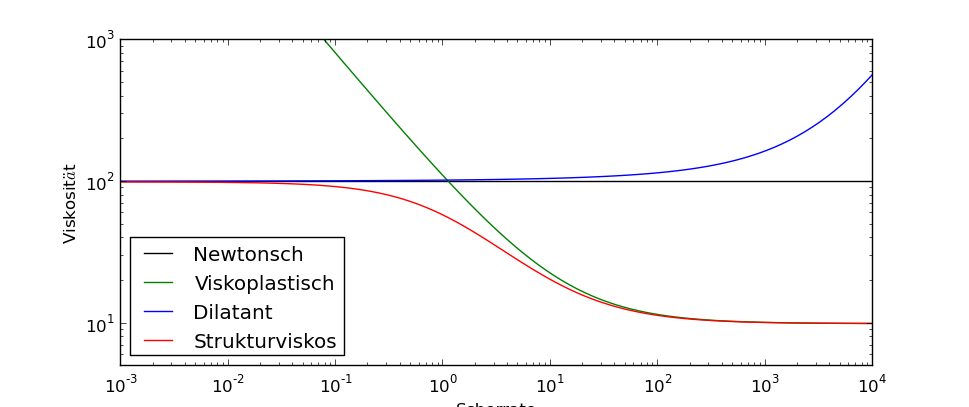
\includegraphics[width=\textwidth]{figures/Fliesskurven.png}
    \caption{Fliesskurven von verschiedenen Fluid-Typen, dargestellt im doppelt logarithmischen Plot.}
    \label{fig:fliessKurven}
\end{figure}
%
\paragraph{Empirische Fliessgesetze}~\\*~\\*
Eine Approximation der Fliesskurven durch analytische Funktionen er\-mög\-licht eine geschlossene Behandlung der Gleichungen, ohne dass auf Tabellendaten oder andere Hilfsmittel zurückgegriffen werden muss.
Solche Modelle enthalten freie Parameter, die an das jeweilige Material angepasst werden müssen.
%
\subparagraph{Newton}
Das Newtonsche Fliessgesetz kann als analytisches Modell mit dem Parameter $\mu$ aufgefasst werden,
\begin{equation}
    \eta = \mu.
    \label{eq:fg:newton}
\end{equation}
%
\subparagraph{Ostwald-de-Waele}
Das einfachste nicht-Newtonsche Fliessgesetz ist das Potenzgesetz nach Ostwald und de~Waele,
\begin{equation}
    \eta=K\gammap^{n-1}.
    \label{eq:fg:potenz}
\end{equation}
Es besitzt zwei Parameter, den Fliessindex \nom[pv:n]{$n$}{Fliessindex in Fliessgesetzen} und den Konsistenzparameter \nom[pv:K]{$K$}{Konsistenzparameter in Fliessgesetzen}. Der Fliessindex entscheidet dabei über das Verhalten des Fluids bei sich ändernder Scherrate (dilatant für $n>1$, strukturviskos für $n<1$ oder Newtonsch für $n=1$). Der Konsistenzparameter ähnelt der Viskosität bei Newtonschen Flüssigkeiten.
%
\subparagraph{Carreau-Yasuda}
Ein Mangel des Ostwald-de-Waele Modells ist das unrealistische Verhalten bei verschwindenden Scherraten, $\gammap\rightarrow 0$. Abhängig von $n$ strebt die Viskosität gegen Unendlich oder gegen Null.
Eine Möglichkeit dies zu beheben, bietet das Carreau-Yasuda-Modell,
\begin{equation}
    \eta=\eta_\infty+\left( \eta_0-\eta_\infty \right)\left[ 1+\left( L\gammap \right)^\alpha \right] ^{\frac{n-1}{\alpha}},
    \label{eq:fg:carreauyasuda}
\end{equation}
durch den Parameter \nom[pv:xc:eta0]{$\eta_0$}{Nullviskosität im Carreau-Yasuda Modell}, der das Grenzverhalten für $\gammap\rightarrow0$ steuert. Des Weiteren beinhaltet das Modell eine Grenzviskosität \nom[pv:xc:etainf]{$\eta_\infty$}{Grenzviskosität im Carreau-Yassuda Modell}, die Zeitkonstante \nom[pv:xc:L]{$L$}{Zeitkonstante im Carreau-Yasuda Modell} und den Fliessindex $n$. Der Parameter \nom[pv:xc:alpha]{$\alpha$}{Parameter im Carreau-Yasuda Modell} steuert den Übergang zwischen Null- und Grenzviskosität.
%
\subparagraph{Bingham}
Ein Bingham Fluid ist ein Material, das erst ab einer Fliessgrenze zu fliessen beginnt, danach aber Newtonsches Verhalten aufweist.
\begin{equation}
    \eta=
    \begin{cases}
        \infty                           &; \tau<\tau_{0}    \quad \text{(Festkörper)}\\
        \frac{\tau-\tau_{0}}{\mu\gammap} &; \tau\geq\tau_{0}
    \end{cases}\quad.
    \label{eq:fg:bingham}
\end{equation}
Dabei ist \nom[pv:xb:tau0]{$\tau_0$}{Fliessgrenze von viskoplastischen Materialien} die Fliessgrenze und $\mu$ die Viskosität im Newtonschen Bereich.
%
\subparagraph{Herschel-Bulkley Modell}
Ein Modell mit einer Fliessgrenze und einem nicht-Newtonschen Verhalten oberhalb dieser Grenze ist das Herschel"=Bulkley"=Modell,
\begin{equation}
    \eta=  \frac{\tau_0}{\gammap}+K\gammap^{n-1}.
    \label{eq:fg:herschelbulkley}
\end{equation}

Die scherratenabhängige Viskosität einiger von Hilti hergestellter Mörtel wurde schon in früheren Arbeiten untersucht
\cite{Marco}.
Die Mörtel zeigen ein viskoplastisches Verhalten, das sich am besten mit dem modifizierten Herschel-Bulkley Modell abbilden lässt:
\begin{equation}
    \label{eq:modHB}
    \eta\left( \gammap \right) = \tau_0 \frac{1-\exp \left( -m\gammap \right)}{\gammap}+K\gammap^{n-1}.
\end{equation}
Die materialabhängigen Parameter sind dabei die Fliessgrenze $\tau_0$, die Konsistenz $K$ und der Fliessindex $n$. Der Parameter $m$ bestimmt das Verhalten des Modells bei sehr kleinen Scherraten und wurde in der vorliegenden Arbeit auf 1000 gesetzt.
%
\subsubsection{Zeitabhängige Spannungen}
Für viele Flüssigkeiten spielt nicht nur der aktuelle Zustand des Fluids eine Rolle, sondern auch die Geschichte der früheren Deformationen. Die konstitutive Gleichung \eqref{eq:Spannungstensor} ist also nicht mehr nur von $\D$ abhängig, sondern auch von der Zeit $t$ und der Verzerrungsgeschichte:
\begin{equation}
    \label{eq:Tviskoelastisch}
    \T\left( \D,t \right) = \underset{s\leq t}{f}\left[ \T\left(\D, s \right),\D\left( s \right) \right].
\end{equation}
%
\paragraph{Maxwell Modell}
Ein Modell, um das Verhalten eines solchen Stoffes zu beschreiben, ist das Maxwell Modell.
Dabei wird das Material als eine Mischung aus einer viskosen Newtonschen Flüssigkeit und einem oder mehreren elastischen Festkörpern beschrieben. Dies geschieht durch eine Kombination aus einem Dämpfer und einer Feder, deren Eigenschaften in Reihe geschaltet sind. 
Eine schematische Darstellung ist in Abbildung~\ref{fig:Maxwell-Material} zu sehen.
Wird nun auf dieses Material eine Kraft in Form einer Spannung ausgeübt, nehmen beide Komponenten einen Teil davon auf, wobei der viskose Dämp"-fer sich unter der Spannung verformt und die Energie als Wärme dissipiert. Die elastische Komponente speichert die Spannung hingegen als elastische Energie und kann diese zu einem späteren Zeitpunkt wieder zurückgeben.
%
\begin{figure}
    \centering
    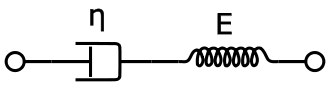
\includegraphics[width=0.5\textwidth]{figures/Maxwell-material.png}
    \caption{Schematische Darstellung eines Maxwell Materialmodells.
    Links der viskose Dämpfer, rechts die elastische Feder. Bildquelle: Wikipedia.}
    \label{fig:Maxwell-Material}
\end{figure}

Die resultierende Differentialgleichung für die Schubspannung $\T$ nimmt folgende Form an:
%
\begin{equation}
    \label{eq:maxwellModell}
    \T + \lambda \frac{\partial\T}{\partial t}=2\eta \D.
\end{equation}
Die Voraussetzung dafür ist, dass das Stoffverhalten als linear angenommen wird. Das bedeutet, es werden nur Verzerrungen mit hinreichend kleiner Amplitude betrachtet. Zusätzlich muss noch die Annahme eines exponentiell schwindenden Gedächtnisses getroffen werden. Das heisst, der Einfluss von Verzerrungen auf die aktuelle Spannung nimmt mit der Zeit exponentiell ab. Dieser Zusammenhang ist in Abbildung~\ref{fig:relaxationszeit} dargestellt.
%
\begin{figure}
    \centering
    \begin{tikzpicture}
        \draw[<->] (0,3) node[left] {$\tau$} -- (0,0) node[below] {0} -- (7,0) node[below] {t};
        \draw[thick] (0,2) to [out=-40, in=180] (6.8,0.05);
        \draw[loosely dashed] (0,2) -- (2.3,0);
        \draw (2.3,-0.1) node[below] {$\lambda$} -- (2.3,0.1);
    \end{tikzpicture}
    \caption{Spannungsrelaxation nach einer plötzlichen Verformung. Je grösser $\lambda$, desto lamgsamer nimmt die Spannung im Fluid ab.}
    \label{fig:relaxationszeit}
\end{figure}
%
\paragraph{Oldroyd-B Modell}
Eine Erweiterung des Maxwell Modells ist das \linebreak Oldroyd"~B Modell, bei dem statt der partiellen die kontravariante Ableitung verwendet wird:\nomenclature[not:oldroyd]{$\overset{\nabla}{\T}$}{Kontravariante (Oldroydsche) Zeitableitung} 
\begin{equation}
    \label{eq:oldroydModell}
    \T + \lambda \overset{\nabla}{\T}=2\eta \D,
\end{equation}
wobei
\begin{equation}
    \label{eq:upperconvectedDerivative}
    \overset{\nabla}{\T} = \frac{D}{Dt}\T-\left[ \nabla \u^T\cdot \T \right]-\left[ \T\cdot \nabla \u \right].
\end{equation}
Diese Modifikation dient dazu, Drehungen und Verzerrungen des Fluides in der Differentialgleichung zu berücksichtigen.
Die Herleitung dieser Ab"-lei"-tung stammt von J.G. Oldroyd \cite{oldroyd}, nach dem auch das Modell benannt ist.

\paragraph{White-Metzner Modell}
Das in dieser Arbeit verwendete Modell für viskoelastische Fluide muss zusätzlich zu der Zeitabhängigkeit auch die starke Scherratenabhängigkeit der Mörtel berücksichtigen können.
Dies bietet das White-Metz"-ner Modell. Dieses ist eine Erweiterung des Oldroyd-B Mo\-del\-les, bei dem zusätzlich $\lambda$ und $\eta$ Funktionen von $\gammap$ sind:
\begin{equation}
    \label{eq:whiteMetznerModell}
    \T + \lambda\left( \gammap \right) \overset{\nabla}{\T}=2\eta\left( \gammap \right) \D.
\end{equation}
Dabei können im Allgemeinen für die Funktionen $\lambda$ und $\eta$ die selben Modelle wie für die nicht zeitabhängigen Gesetze verwendet werden.
In dieser Arbeit wurde für $\eta$ das schon bewährte modifizierte Herschel-Bulkley Modell \eqref{eq:modHB} implementiert.
Die Relaxationszeit weist für die untersuchten Mörtel, abhängig von der Scherrate, zwei Plateaus auf; bei hinreichend kleiner und grosser Scherrate. Der Übergang  verläuft exponentiell, wie in Abbildung~\ref{fig:carreauYasudaAnnotated} gezeigt.
Als beschreibende Funktion für $\lambda$ wird daher auf Empfehlung des Rheologiespezialisten von Hilti das Carreau-Yasuda Modell \eqref{eq:fg:carreauyasuda} verwendet.
%
\begin{figure}[h]
    \centering
    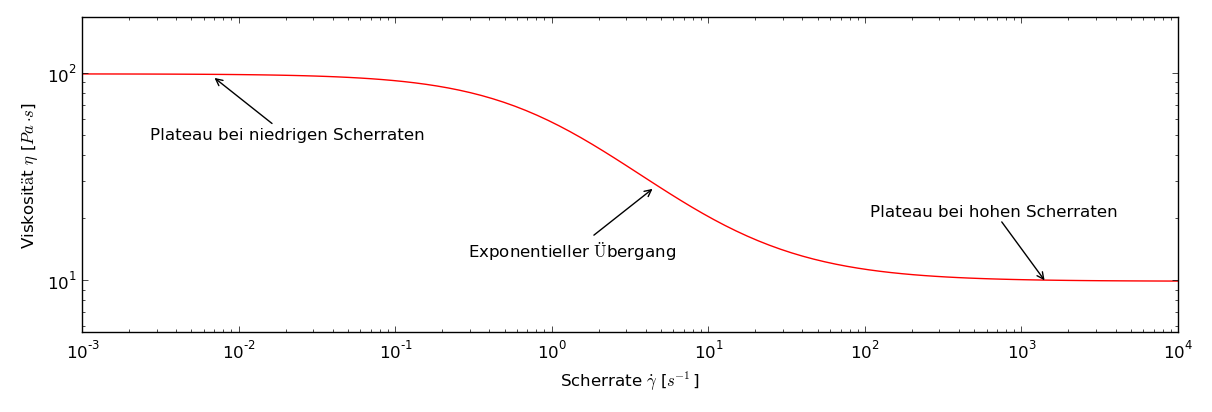
\includegraphics[width=\textwidth]{figures/CarreauYasudaAnnotated.png}
    \caption{Beispielkurve des Carreau-Yasuda Modells.}
    \label{fig:carreauYasudaAnnotated}
\end{figure}
